\section{Implementación computacional de las bases discretas de Legendre}
\label{Implementación computacional de las bases discretas de Legendre en Python}

Haciendo uso de
la fórmula establecida en el teorema
\ref{teo: expresión analítica de BON de Legendre}
y las simetrías exploradas en el capítulo
\ref{section: sobre simetrias en las entradas de los poliomios discretos de Legendre}, definiremos un
algoritmo para calcular
las bases de Legendre discretas. Para implementarlo, lo escribiremos
en Python. 
El input y output del algoritmo deseado son como siguen:


\begin{itemize}
\item \textbf{Input}: la dimensión requerida $n \geq 2$, variable
de tipo \code{int}. 
\item \textbf{Output}: lista con $n$ entradas,
siendo la $k-$ésima entrada (con $0 \leq k \leq n-1$)
una lista que contiene las $n$ entradas del
vector $\cali{L}^{n,k}$.
\end{itemize}

\begin{figure}[H]
	\sidecaption{
		Se ilustran el input y el output
		esperados del algoritmo para $n=5$. En los scripts
		que escribimos no se pidió redondeo a cuatro decimales.
	\label{fig: input y output deseados}
	}
	\centering
	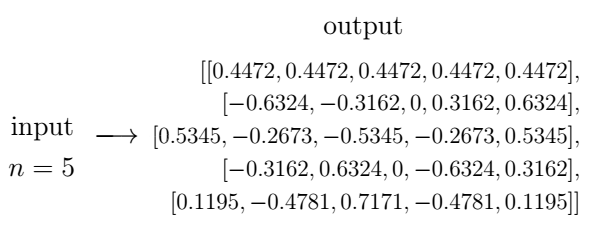
\includegraphics[scale=0.7]{7En_1} 
\end{figure}	

\subsection{Análisis de la expresión de los PDL}
Sean $n \in \IN$, $0 \leq k \leq n-1$.
Veamos cómo usar lo que sabemos para calcular eficientemente
al vector $\cali{L}^{n,k}$ o, equivalentemente, para calcular
cada una de sus $n$ entradas, que son los números reales
$\cali{L}^{n,k}_{m}$, con $0 \leq m \leq n-1$.

Conviene reescribir la expresión
\eqref{eq0: 6En} resaltando con colores el papel que juegan
la dimensión $n$, el grado $k$ y la posición $m$ en la fórmula
para $\cali{L}^{n,k}_{m}$:

\begin{equation}
\label{eq1: 6En}
\cali{L}^{
{\color{ameCyanO}{n}},{\color{ameVerde}{k}}}_{\color{ameGris}{m}}= 
(-1)^{{\color{ameVerde}{k}}} 
\sqrt{\frac{(2
{\color{ameVerde}{k}}+1)(
{\color{ameCyanO}{n}}-1)^{(
{\color{ameVerde}{k}})}}{(
{\color{ameCyanO}{n}}+
{\color{ameVerde}{k}})^{(
{\color{ameVerde}{k}}+1)}}}
\suma{j=0}{
{\color{ameVerde}{k}}}{(-1)^{j}\binom{
{\color{ameVerde}{k}}}{j}\binom{
{\color{ameVerde}{k}}+j}{j}
\frac{{\color{ameGris}{m}}^{(j)}}{(
{\color{ameCyanO}{n}}-1)^{(j)}}}.
\end{equation}

Recuerde el concepto de fading factorial
definido en \ref{def: fading factorial}.
Observe ahora que, en la expresión \eqref{eq1: 6En},
aparecen cuatro fading factorials;
\begin{itemize}
\item $(n-1)^{(k)}$, que nunca es cero, pues $n-1 \geq k$
siempre ocurre,
\item $(n+k)^{(k+1)}$, que nunca es cero, pues $n+k \geq k+1$
siempre ocurre,
\item $(n-1)^{(j)}$ que, por ocurrir $j \leq k \leq n-1$, 
nunca es cero, y
\item $m^{(j)}$, que no es cero si y sólo si $j \leq m$;
\end{itemize}
según este último punto, algunos de los sumandos
considerados en la sumatoria 
en \eqref{eq1: 6En} pueden ser cero; podemos
ajustar el limite superior de la sumatoria y llegar así a que
\begin{equation}
\label{eq2: 6En}
\cali{L}^{
{\color{ameCyanO}{n}},{\color{ameVerde}{k}}}_{\color{ameGris}{m}}= 
(-1)^{{\color{ameVerde}{k}}} 
\sqrt{\frac{(2
{\color{ameVerde}{k}}+1)(
{\color{ameCyanO}{n}}-1)^{(
{\color{ameVerde}{k}})}}{(
{\color{ameCyanO}{n}}+
{\color{ameVerde}{k}})^{(
{\color{ameVerde}{k}}+1)}}}
\suma{j=0}{
min(
{\color{ameVerde}{k}},
{\color{ameGris}{m}})
}{
{(-1)^{j}\binom{
{\color{ameVerde}{k}}}{j}\binom{
{\color{ameVerde}{k}}+j}{j}
\frac{{\color{ameGris}{m}}^{(j)}}{(
{\color{ameCyanO}{n}}-1)^{(j)}}}.
},
\end{equation}

Podemos también usar la definición de fading factorial
para reescribir \eqref{eq2: 6En}
en términos de factoriales
como sigue:


\begin{equation}
\label{eq5: 6En}
\cali{L}^{
{\color{ameCyanO}{n}},{\color{ameVerde}{k}}}_{\color{ameGris}{m}}= 
A_{
{\color{ameCyanO}{n}},
{\color{ameVerde}{k}}
}
\suma{j=0}{
min(
{\color{ameVerde}{k}},
{\color{ameGris}{m}})}
{B_{
{\color{ameCyanO}{n}},
{\color{ameVerde}{k}},
{\color{ameGris}{m}},j
}
},
\end{equation}
donde

\begin{equation}
\label{eq3: 6En}
A_{
{\color{ameCyanO}{n}},
{\color{ameVerde}{k}}
}:=
(-1)^{{\color{ameVerde}{k}}} 
({\color{ameCyanO}{n}}-1)!
\sqrt{\frac{(2
{\color{ameVerde}{k}}+1)}
{(
{\color{ameCyanO}{n}}-
({\color{ameVerde}{k}}+1))!
(
{\color{ameCyanO}{n}} + {\color{ameVerde}{k}}
)!
}},
\end{equation}
y

\begin{equation}
\label{eq4: 6En}
B_{
{\color{ameCyanO}{n}},
{\color{ameVerde}{k}},
{\color{ameGris}{m}},j
}:=
(-1)^{j}
\frac{
{\color{ameGris}{m}}!
}{
({\color{ameCyanO}{n}}-1)!
}
\frac{
({\color{ameVerde}{k}} + j) !
({\color{ameCyanO}{n}}-(j+1))!
}{
(j!)^{2}
({\color{ameVerde}{k}}-j)!
({\color{ameGris}{m}}-j)!
}.
\end{equation}



Usando las fórmulas \eqref{eq5: 6En}, 
\eqref{eq3: 6En} y \eqref{eq4: 6En} junto con las
simetrías estudiadas en la sección 
\ref{section: sobre simetrias en las entradas de los poliomios discretos de Legendre}, podemos escribir con facilidad el algoritmo deseado.

\section{Pseudocódigos algoritmos usados para calcular las BDL}
A continuación mostramos los pseudocódigos para calcular 
los polinomios discretos de Legendre.

Las implementaciones en Python de todos estos algoritmos
se compartieron en \TODO{referencia.}

\begin{itemize}
\item Damos los algoritmos \textbf{sumandoV1} y 
\textbf{sumandoV2} (c.f. \ref{alg: sumandoV1},
\ref{alg: sumandoV2}) para calcular el número
\begin{equation}
\label{eq0: 1Abril}
B_{n, k, m, j};
\end{equation}
el primero usa directamente la fórmula \eqref{eq4: 6En},
mientras que en el segundo 
simplificamos los factoriales que
aparecen en la definición \eqref{eq4: 6En}
de $B_{n,k,m,j}$
para llegar a la expresión
\[
(-1)^{j}
\frac{m!}{(n-1)!}
 \frac{(k+j)!(n-j-1)!}{(j!)^{2}(k-j)!(m-j)!}
= (-1)^{j}
\frac{\left( \producto{\mu=m-j+1}{m}{\mu} \right)
\left( \producto{\mu=k-j+1}{k+1}{\mu} \right)
}{
\left( \producto{\mu=n-j}{n-1}{\mu} \right)
\left( \producto{\mu=n-j}{n-1}{\mu} \right)^{2}
}.
\] 

\item Damos dos algoritmos \textbf{sumatoriaV1}
y \textbf{sumatoriaV2} (c.f. \ref{alg: sumatoriaV1}
y c.f. \ref{alg: sumatoriaV2}) para calcular a la suma
\begin{equation}
\label{eq1: 1Abril}
\suma{j=0}{min(k,m)}{B_{n, k, m, j}};
\end{equation}
observe en la definición de estos que 
\textbf{sumatoriaV1} hace referencia a
\textbf{sumandoV1}, mientras que \textbf{sumatoriaV2}
hace referencia a \textbf{sumandoV2}


\item Los algoritmos 
\textbf{baseLegendre$\_$dimImpar} y
\textbf{baseLegendre$\_$dimPar} 
(c.f. \ref{alg: legendre impar} y \ref{alg: legendre par} )
que sirven para calcular, usando ya sea el algoritmo
\textbf{sumatoriaV1} o \textbf{sumatoriaV2},
la base de Legendre discreta de dimensión $n$; se usa el primero
si $n$ es impar y el segundo si $n$ es par.
Las lineas 10 de estos 
algoritmos se justifican,
respectivamente, con los teoremas 
\ref{prop: simetrias en dimensiones impares}
y \ref{prop: simetrias en dimensiones pares}.
Por último, tenemos el sencillo algoritmo \textbf{calculo$\_$base},
que, en base a la paridad de la dimensión $n$, decide si usar
el algoritmo \ref{alg: legendre impar} o el \ref{alg: legendre par}
para calcular la BDL de dimensión $n$.
\end{itemize}

Para los pseudocódigos usamos las siguiente abreviaciones:

\begin{itemize}
	\item \textit{APPEND(A,t)} donde $A$ es una lista y $t$ es un elemento
	significa ``agregar $t$ al final de la lista $A$''.
	\item \textit{CONCATENATE(A,B)}, donde $A$ y $B$ son listas, significa
	concatenar $A$ con $B$.
	\item \textit{PRODUCT(A)}, donde $A$ es una lista cuyas entradas
	son todas variables de tipo \code{float}, significa ``calcular el producto
	de todos los elementos de $A$''. Si $A$ es vacía, $PRODUCT(A)$ es uno.
	\item \textit{SUM(A)}, donde $A$ es una lista cuyas entradas
	son todas variables de tipo \code{float}, significa ``calcular la suma
	de todos los elementos de $A$''. 
	\item \textit{CEIL(a)}, donde $a$ es una variable de tipo \code{float}, significa
	``calcular $\lceil a \rceil$''.
\end{itemize}

\begin{algorithm}
\caption{$sumandoV1$}\label{alg: sumandoV1}
\begin{algorithmic} [1]
\REQUIRE $n$, $k$, $m$, $j$, todas de tipo int, con $n \geq 2$, 
$0 \leq k, m \leq n-1$, $0 \leq j \leq min(k,m)$
\ENSURE El número \eqref{eq0: 1Abril}
\RETURN $\frac{(k+j)! * (n-j-1)! }{(j!)^{2}* (k-j)! * (m-j)!}$
\end{algorithmic}
\end{algorithm}

\begin{algorithm}
\caption{$sumandoV2$}\label{alg: sumandoV2}
\begin{algorithmic} [1]
\REQUIRE $n$, $k$, $m$, $j$, todas de tipo int, con $n \geq 2$, 
$0 \leq k, m \leq n-1$, $0 \leq j \leq min(k,m)$
\ENSURE El número \eqref{eq0: 1Abril}
\STATE $B1, B2, B3, B4 \leftarrow []$
\FOR {$t=m-j+1$ a $t=m$} 
\STATE $APPEND(B1, t)$
\ENDFOR
\FOR {$t=k-j+1$ a $t=k+j$} 
\STATE $APPEND(B2, t)$
\ENDFOR
\FOR {$t=n-j$ a $t=n-1$} 
\STATE $APPEND(B3, t)$
\ENDFOR
\FOR {$t=1$ a $t=j$} 
\STATE $APPEND(B4, t)$
\ENDFOR
\STATE $num \leftarrow CONCATENATE(B1, B2)$
\STATE $den \leftarrow CONCATENATE(B3, B4)$
\STATE $den \leftarrow CONCATENATE(den, B4)$
\STATE $numerador = PRODUCT(num)$
\STATE $denominador = PRODUCT(den)$
\RETURN $numerador/denominador$
\end{algorithmic}
\end{algorithm}



\begin{algorithm}
\caption{$sumatoriaV1$}\label{alg: sumatoriaV1}
\begin{algorithmic} [1]
\REQUIRE $n$, $k$, $m$, $j$, todas de tipo int, con $n \geq 2$, 
$0 \leq k, m \leq n-1$, $0 \leq j \leq min(k,m)$
\ENSURE La suma \eqref{eq1: 1Abril}

\STATE $limite \leftarrow minimo(m,k)$
\STATE $factor \leftarrow \frac{m!}{(n-1)!}$
\STATE $sumandos\_pares \leftarrow []$
\STATE $sumandos\_impares \leftarrow []$
\FOR {$j=0$ a $j=limite$ y $j$ par} 
\STATE $APPEND$($sumandos\_pares$, $sumandoV1(n,k,m,j)$)
\ENDFOR
\FOR {$j=0$ a $j=limite$ y $j$ impar} 
\STATE $APPEND$($sumandos\_impares$, $sumandoV1(n,k,m,j)$)
\ENDFOR
\STATE $suma\_pares \leftarrow SUM(sumandos\_pares)$
\STATE $suma\_impares \leftarrow SUM(sumandos\_impares)$
\RETURN $factor * (suma\_pares - suma\_impares)$
\end{algorithmic}
\end{algorithm}

\begin{algorithm}
\caption{$sumatoriaV2$}\label{alg: sumatoriaV2}
\begin{algorithmic} [1]
\REQUIRE $n$, $k$, $m$, $j$, todas de tipo int, con $n \geq 2$, 
$0 \leq k, m \leq n-1$, $0 \leq j \leq min(k,m)$
\ENSURE La suma \eqref{eq1: 1Abril}

\STATE $limite \leftarrow minimo(m,k)$
\STATE $sumandos\_pares \leftarrow []$
\STATE $sumandos\_impares \leftarrow []$
\FOR {$j=0$ a $j=limite$ y $j$ par} 
\STATE $APPEND$($sumandos\_pares$, $sumandoV2(n,k,m,j)$)
\ENDFOR
\FOR {$j=0$ a $j=limite$ y $j$ impar} 
\STATE $APPEND$($sumandos\_impares$, $sumandoV2(n,k,m,j)$)
\ENDFOR
\STATE $suma\_pares \leftarrow SUM(sumandos\_pares)$
\STATE $suma\_impares \leftarrow SUM(sumandos\_impares)$
\RETURN $suma\_pares - suma\_impares$
\end{algorithmic}
\end{algorithm}


%-----------------------------------------------------------------

\begin{algorithm}
\caption{baseLegendre$\_$dimImpar}\label{alg: legendre impar}
\begin{algorithmic}[1] 
\REQUIRE $n$, variable de tipo int, $n \geq 2, \hspace{0.1cm} n \equiv 1 \hspace{0.1cm} (mod \hspace{0.1cm} 2)$, 'sumatoria' es una de las dos funciones definidas en los algoritmos
\ref{alg: sumatoriaV1} y \ref{alg: sumatoriaV2}.
\ENSURE lista cuyos elementos son $n$ listas, conteniendo
la $k-$ésima lista las $n$ entradas del polinomio discreto de Legendre de
grado $k$ y dimensión $n$.
%\ENSURE $y = x^n$
\STATE $M \leftarrow CEIL(n/2)$
\STATE $base\_legendre=[ \hspace{0.2cm} ]$ 
\STATE $signo \leftarrow 1$ 
\FOR {$k=0$ a $k=n-1$} 
\STATE $A\_nk \leftarrow signo * (n-1)!*
\sqrt{\frac{
2k+1
}{
(n-k-1)!*(n+k)!
}}$

\STATE $vector\_legendre \leftarrow [ 0, \ldots , 0]$ \COMMENT{Lista con $n$ ceros} 
\FOR {$m=0$ a $m=M-2$} 
\STATE $entrada \leftarrow A\_nk * sumatoria(n,k,m)$
\STATE $vector\_legendre[m] \leftarrow entrada$ 
\STATE $vector\_legendre[n-m-1] \leftarrow signo*entrada$ 
\ENDFOR

\IF{$k \equiv 1 \hspace{0.1cm} (mod \hspace{0.1cm} 2)$}
\STATE $vector\_legendre[M-1] \leftarrow 0$
\ELSE
\STATE $vector\_legendre[M-1] \leftarrow A\_nk * sumatoria(n,k,M-1)$
\ENDIF
\STATE $APPEND(base\_legendre, vector\_legendre)$
\STATE $signo \leftarrow signo * -1$
\ENDFOR
\RETURN $base\_legendre$
\end{algorithmic}
\end{algorithm}



\begin{algorithm}
\caption{baseLegendre$\_$dimPar}\label{alg: legendre par}
\begin{algorithmic} [1]
\REQUIRE $n$, variable de tipo int, $n \geq 2, \hspace{0.1cm} n \equiv 0 \hspace{0.1cm} (mod \hspace{0.1cm} 2)$, 'sumatoria' es una de las dos funciones definidas en los algoritmos
\ref{alg: sumatoriaV1} y \ref{alg: sumatoriaV2}.
\ENSURE lista cuyos elementos son $n$ listas, conteniendo
la $k-$ésima lista las $n$ entradas del polinomio discreto de Legendre de
grado $k$ y dimensión $n$.


\STATE $M \leftarrow CEIL(n/2)$
\STATE $base\_legendre=[ \hspace{0.2cm} ]$ 
\STATE $signo \leftarrow 1$ 

\FOR {$k=0$ a $k=n-1$} 
\STATE $A\_nk \leftarrow signo * (n-1)!*
\sqrt{\frac{
2k+1
}{
(n-k-1)!*(n+k)!
}}$

\STATE $vector\_legendre \leftarrow [ 0, \ldots , 0]$ \COMMENT{Lista con $n$ ceros} 
\FOR {$m=0$ a $m=M-1$} 
\STATE $entrada \leftarrow A\_nk * sumatoria(n,k,m)$
\STATE $vector\_legendre[m] \leftarrow entrada$ \COMMENT{Agregamos en la $m-$ésima posición}
\STATE $vector\_legendre[n-m-1] \leftarrow signo *entrada\_legendre$
\ENDFOR

\STATE $APPEND(base\_legendre, vector\_legendre)$
\STATE $signo \leftarrow signo * -1$
\ENDFOR
\RETURN $base\_legendre$
\end{algorithmic}
\end{algorithm}



\begin{algorithm}
\caption{calculo$\_$base}\label{alg: legendre}
\begin{algorithmic} [1]
\REQUIRE $n$, variable de tipo int, $n \geq 2$, función ``sumatoria''
\ENSURE lista cuyos elementos son $n$ listas, conteniendo
la $k-$ésima lista las $n$ entradas del polinomio discreto de Legendre de
grado $k$ y dimensión $n$.

\IF{$n \equiv 0 \hspace{0.1cm} (mod \hspace{0.1cm} 2)$}
\STATE $base\_legendre\_dimPar(n)$
\ELSE
\STATE $base\_legendre\_dimImpar(n)$
\ENDIF
\end{algorithmic}
\end{algorithm}


